%%% The main file. It contains definitions of basic parameters and includes all other parts.

%% Settings for single-side (simplex) printing
% Margins: left 40mm, right 25mm, top and bottom 25mm
% (but beware, LaTeX adds 1in implicitly)
\documentclass[12pt,a4paper]{report}
\setlength\textwidth{145mm}
\setlength\textheight{247mm}
\setlength\oddsidemargin{15mm}
\setlength\evensidemargin{15mm}
\setlength\topmargin{0mm}
\setlength\headsep{0mm}
\setlength\headheight{0mm}
% \openright makes the following text appear on a right-hand page
\let\openright=\clearpage

%% Settings for two-sided (duplex) printing
% \documentclass[12pt,a4paper,twoside,openright]{report}
% \setlength\textwidth{145mm}
% \setlength\textheight{247mm}
% \setlength\oddsidemargin{14.2mm}
% \setlength\evensidemargin{0mm}
% \setlength\topmargin{0mm}
% \setlength\headsep{0mm}
% \setlength\headheight{0mm}
% \let\openright=\cleardoublepage

%% Generate PDF/A-2u
\usepackage[a-2u]{pdfx}

%% Character encoding: usually latin2, cp1250 or utf8:
\usepackage[utf8]{inputenc}

%% Prefer Latin Modern fonts
\usepackage{lmodern}

%% Further useful packages (included in most LaTeX distributions)
\usepackage{amsmath}           % extensions for typesetting of math
\usepackage{amsfonts}          % math fonts
\usepackage{amsthm}            % theorems, definitions, etc.
\usepackage{bbding}            % various symbols (squares, asterisks, ...)
\usepackage{bm}                % boldface symbols (\bm)
\usepackage{graphicx}          % embedding of pictures
\usepackage{fancyvrb}          % improved verbatim environment
\usepackage[square]{natbib}            % citation style AUTHOR (YEAR), or AUTHOR [NUMBER]
\usepackage[nottoc]{tocbibind} % makes sure that bibliography and the lists
                               % of figures/tables are included in the table
                               % of contents
\usepackage{dcolumn}           % improved alignment of table columns
\usepackage{booktabs}          % improved horizontal lines in tables
\usepackage{paralist}          % improved enumerate and itemize
\usepackage{xcolor}            % typesetting in color
\usepackage{url}
\usepackage{hyperref}
\usepackage{nameref}
\usepackage{macros}
\usepackage{caption}
\usepackage{subcaption}
\usepackage{amsmath}
\usepackage{algorithm}
\usepackage{algpseudocode}
\usepackage{listings}
\usepackage{xcolor}
\usepackage[capitalise]{cleveref}


%%% Basic information on the thesis

% Thesis title in English (exactly as in the formal assignment)
\def\ThesisTitle{Evaluating Point Cloud Rendering Approaches for Camera Pose Verification}

% Author of the thesis
\def\ThesisAuthor{Tomáš Kremel}

% Year when the thesis is submitted
\def\YearSubmitted{2022}

% Name of the department or institute, where the work was officially assigned
% (according to the Organizational Structure of MFF UK in English,
% or a full name of a department outside MFF)
\def\Department{Department of Algebra}

% Department of Theoretical Computer Science and Mathematical Logic
% Is it a department (katedra), or an institute (ústav)?
\def\DeptType{Department}

% Thesis supervisor: name, surname and titles
\def\SupervisorA{doc. Ing. Tomáš Pajdla, Ph.D.}
\def\SupervisorB{Torsten Sattler, Dr. rer. nat.}

% Supervisor's department (again according to Organizational structure of MFF)
\def\SupervisorsDepartment{Department of Algebra}

% Study programme and specialization
\def\StudyProgramme{Computer Science}
\def\StudyBranch{Artificial Intelligence}

% An optional dedication: you can thank whomever you wish (your supervisor,
% consultant, a person who lent the software, etc.)
\def\Dedication{%
I would like to express my gratitude and appreciation to my supervisors,
for their suggestions, great support, and inexhaustible patience while
I was finding motivation. I would also like to thank The Czech Institute
of Informatics, Robotics, and Cybernetics for providing me with all the
necessary GPU resources required for computations. Further, I would like
to recognize my friends Tomáš Souček and Vojtěch Kužel for their consultations.
Finally, my admiration and credit go to my wife, without whom this thesis
would not be a reality.
}

% Abstract (recommended length around 80-200 words; this is not a copy of your thesis assignment!)
\def\Abstract{%
Visual localization is the problem of estimating the 6~degrees of freedom
(DoF) camera pose from which a query image was taken relative to a known
reference scene representation. It is the key for applications such as
Augmented, Mixed, and Virtual Reality, as well as autonomous robotics
such as drones or self-driving cars.

This thesis focuses on the pose verification and ranking step of a visual
localization pipeline that uses 3D point clouds and 2D-3D correspondences
between the query image and 3D scene points for candidate camera poses
estimations. The thesis explores point cloud rendering approaches as they
are utilized in the verification step – the render of the discretized
scene from a given candidate position is compared to the actual query
image to asses if the given couple depicts the same place.

One of the main challenges of such rendering is occlusion handling. Due
to the sparsity of points employed for otherwise continuous real world
representation, information about what lies in the front and what is
hidden can be easily lost when projected to the 2D image. Rendering
approaches explored in this thesis focus on the challenge directly or
as a component for training a novel view synthesis DNN-based renderer.
Rendering influence on localization performance is investigated.
}

% 3 to 5 keywords (recommended), each enclosed in curly braces
\def\Keywords{%
{point clouds,} {rendering,} {neural rendering,} {localization}
}

%% The hyperref package for clickable links in PDF and also for storing
%% metadata to PDF (including the table of contents).
%% Most settings are pre-set by the pdfx package.
\hypersetup{unicode}
\hypersetup{breaklinks=true}

% Definitions of macros (see description inside)
% %%% This file contains definitions of various useful macros and environments %%%
%%% Please add more macros here instead of cluttering other files with them. %%%

%%% Minor tweaks of style

% These macros employ a little dirty trick to convince LaTeX to typeset
% chapter headings sanely, without lots of empty space above them.
% Feel free to ignore.

\ProvidesPackage{macros}[2022/01/10 v1.0 Thesis macros]

\makeatletter
\def\@makechapterhead#1{
  {\parindent \z@ \raggedright \normalfont
   \Huge\bfseries \thechapter. #1
   \par\nobreak
   \vskip 20\p@
}}
\def\@makeschapterhead#1{
  {\parindent \z@ \raggedright \normalfont
   \Huge\bfseries #1
   \par\nobreak
   \vskip 20\p@
}}
\makeatother

% This macro defines a chapter, which is not numbered, but is included
% in the table of contents.
\def\chapwithtoc#1{
\chapter*{#1}
\addcontentsline{toc}{chapter}{#1}
}

% Draw black "slugs" whenever a line overflows, so that we can spot it easily.
\overfullrule=1mm

%%% Macros for definitions, theorems, claims, examples, ... (requires amsthm package)

\theoremstyle{plain}
\newtheorem{thm}{Theorem}
\newtheorem{lemma}[thm]{Lemma}
\newtheorem{claim}[thm]{Claim}

\theoremstyle{plain}
\newtheorem{defn}{Definition}

\theoremstyle{remark}
\newtheorem*{cor}{Corollary}
\newtheorem*{rem}{Remark}
\newtheorem*{example}{Example}

%%% An environment for proofs

\newenvironment{myproof}{
  \par\medskip\noindent
  \textit{Proof}.
}{
\newline
\rightline{$\qedsymbol$}
}

%%% An environment for typesetting of program code and input/output
%%% of programs. (Requires the fancyvrb package -- fancy verbatim.)

\DefineVerbatimEnvironment{code}{Verbatim}{fontsize=\small, frame=single}

%%% The field of all real and natural numbers
\newcommand{\R}{\mathbb{R}}
\newcommand{\N}{\mathbb{N}}

\newcommand{\CC}{C\nolinebreak\hspace{-.05em}\raisebox{.4ex}{\tiny\bf +}\nolinebreak\hspace{-.10em}\raisebox{.4ex}{\tiny\bf +}}

%%% Useful operators for statistics and probability
\DeclareMathOperator{\pr}{\textsf{P}}
\DeclareMathOperator{\E}{\textsf{E}\,}
\DeclareMathOperator{\var}{\textrm{var}}
\DeclareMathOperator{\sd}{\textrm{sd}}

%%% Transposition of a vector/matrix
\newcommand{\T}[1]{#1^\top}

%%% Various math goodies
\newcommand{\goto}{\rightarrow}
\newcommand{\gotop}{\stackrel{P}{\longrightarrow}}
\newcommand{\maon}[1]{o(n^{#1})}
\newcommand{\abs}[1]{\left|{#1}\right|}
\newcommand{\dint}{\int_0^\tau\!\!\int_0^\tau}
\newcommand{\isqr}[1]{\frac{1}{\sqrt{#1}}}
\newcommand*{\fullref}[1]{\hyperref[{#1}]{\cref*{#1}: \nameref*{#1}}}

%%% Various table goodies
\newcommand{\pulrad}[1]{\raisebox{1.5ex}[0pt]{#1}}
\newcommand{\mc}[1]{\multicolumn{1}{c}{#1}}

%%% Other macros
\renewcommand{\labelitemi}{\footnotesize{\textbullet}}
\newcommand{\uv}[1]{``#1''}
\newcommand{\footnotei}[2]{%
\setbox0\hbox{#1}%
\copy0%
\hspace{-\wd0}%
\footnote{#2}%
}

\newcommand{\gear}[6]{%
  (0:#2)
  \foreach \i [evaluate=\i as \n using {\i-1)*360/#1}] in {1,...,#1}{%
    arc (\n:\n+#4:#2) {[rounded corners=1.5pt] -- (\n+#4+#5:#3)
    arc (\n+#4+#5:\n+360/#1-#5:#3)} --  (\n+360/#1:#2)
  }%
  (0,0) circle[radius=#6]
}

\makeatletter
\newcommand{\gettikzxy}[3]{%
  \tikz@scan@one@point\pgfutil@firstofone#1\relax
  \edef#2{\the\pgf@x}%
  \edef#3{\the\pgf@y}%
}
\makeatother


% Title page and various mandatory informational pages
\begin{document}
%%% Title page of the thesis and other mandatory pages

%%% Title page of the thesis

\pagestyle{empty}
\hypersetup{pageanchor=false}
\begin{center}

\centerline{\mbox{\includegraphics[width=166mm]{../graphics/logo-en.pdf}}}

\vspace{-8mm}
\vfill

{\bf\Large MASTER THESIS}

\vfill

{\LARGE\ThesisAuthor}

\vspace{15mm}

{\LARGE\bfseries\ThesisTitle}

\vfill

\Department

\vfill

{
\centerline{\vbox{\halign{\hbox to 0.45\hsize{\hfil #}&\hskip 0.5em\parbox[t]{0.45\hsize}{\raggedright #}\cr
Supervisor of the master thesis:&\Supervisor \cr
\noalign{\vspace{2mm}}
Study programme:&\StudyProgramme \cr
\noalign{\vspace{2mm}}
Study branch:&\StudyBranch \cr
}}}}

\vfill

% Zde doplňte rok
Prague \YearSubmitted

\end{center}

\newpage

%%% Here should be a bound sheet included -- a signed copy of the "master
%%% thesis assignment". This assignment is NOT a part of the electronic
%%% version of the thesis. DO NOT SCAN.

%%% A page with a solemn declaration to the master thesis

\openright
\hypersetup{pageanchor=true}
\pagestyle{plain}
\pagenumbering{roman}
\vglue 0pt plus 1fill

\noindent
I declare that I carried out this master thesis independently, and only with the cited
sources, literature and other professional sources. It has not been used to obtain another
or the same degree.

\medskip\noindent
I understand that my work relates to the rights and obligations under the Act No.~121/2000 Sb.,
the Copyright Act, as amended, in particular the fact that the Charles
University has the right to conclude a license agreement on the use of this
work as a school work pursuant to Section 60 subsection 1 of the Copyright~Act.

\vspace{10mm}

\hbox{\hbox to 0.5\hsize{%
In \hbox to 6em{\dotfill} date \hbox to 6em{\dotfill}
\hss}\hbox to 0.5\hsize{\dotfill\quad}}
\smallskip
\hbox{\hbox to 0.5\hsize{}\hbox to 0.5\hsize{\hfil Author's signature\hfil}}

\vspace{20mm}
\newpage

%%% Dedication

\openright

\noindent
\Dedication

\newpage

%%% Mandatory information page of the thesis

\openright

\vbox to 0.5\vsize{
\setlength\parindent{0mm}
\setlength\parskip{5mm}

Title:
\ThesisTitle

Author:
\ThesisAuthor

\DeptType:
\Department

Supervisor:
\Supervisor, \SupervisorsDepartment

Abstract:
\Abstract

Keywords:
\Keywords

\vss}

\newpage

\openright
\pagestyle{plain}
\pagenumbering{arabic}
\setcounter{page}{1}


%%% A page with automatically generated table of contents of the master thesis

\tableofcontents

%%% Each chapter is kept in a separate file
\chapter*{Introduction}
\addcontentsline{toc}{chapter}{Introduction}


\chapter{Visual Localization} \label{chap:visual_loc}

As stated in~\nameref{intro}, visual localization is the task of finding
the position of a camera that took a query photo relative to a reference scene
representation, and it is one of the fundamental problems in computer vision.

Compared to network-based localization methods, such as GNSS, visual localization,
even though being able to work in network-denied environments, comes with its own
set of problems that any successful method must consider. For both outdoor and
indoor localization, to which the field is typically separated due to different
localization complexity, illumination changes throughout the day and artificial lighting
influence present in the environment's representation data pose one class of such problems.
Further, it must cope with transient dynamic objects that can be present in both query
and database data, possibly occluding important feature-rich areas but having nothing
to do with the long-term visual appearance of the given location. Outdoors, seasonal and
weather-caused changes must be handled as well. For indoors, more problems stem from
textureless areas such as walls, ceilings, and floors; from repetition and symmetry
on both the global level with corridors, for example, and the local level, such as door handles.
Also, compared to outside, with typically longer distances between objects, inside small change
of viewing position leads to a vastly different view.

In this chapter, we present previous work on the matter and describe the InLoc method
explored in the thesis, explaining why this very method is chosen.

\section{Related work}

There are three main method categories for visual localization, as of \citet{torsten2018},
\citet{torsten2019}, \citet{torsten2021}, \citet{naverlabs}: methods based on structure,
image retrieval, and pose regression.

\subsubsection*{Structure-based methods}

Structure-based methods are the traditional way of estimating poses where a 3D model (the \emph{structure}) is
pre-created in order to later find 2D-3D correspondences.

% used https://arxiv.org/pdf/2007.13867.pdf
The 3D model is typically created by
Structure-from-Motion~\citep{SfM, schoenberger2016mvs}, by computing local sparse features (keypoints with descriptors,
\citet{LoweLocalization} used SIFT~\citep{SIFT} descriptor, \citet{PreSIFT} was pre-SIFT, using image rectification)
per database image with known focal length, match them against each other across images, and triangulate resulting 3D points
from these matches. Since the model already contains pre-computed features, matching against
a query image's features can then be performed. Since the 2D-3D matches are determined, the camera pose
is computed using the perspective-n-point (PNP) solver~\citep{PnP}. Because of the possible presence of outlier matches,
a RANSAC loop~\citep{RANSAC} is utilized to increase robustness. Other examples of this approach are~\citet{2D3D, 2D3D_2}.

With the growing size of a 3D point cloud, the runtime gets prolonged. To mitigate matching speed deterioration,
these methods also get paired with image retrieval, described next, to find the most
relevant images from the SFM model. Examples of these methods
are~\citet{InLoc, InLocRevisited, MegLoc}.

\subsubsection*{Image retrieval-based methods}

Image retrieval can be used to speed up the structure-based method family and make mapping
and localization more robust. That is because the restriction of matching to the parts of the scene visible in the given query photo
helps to avoid global ambiguities in the scene, e.g., caused by similar structures found in unrelated parts
of a scene~\citep{InLocRevisited}. It can also be used on its own for a closely related task to visual
localization called place recognition, which strives to find the approximate location of a query photo within a database
of geo-tagged images. Unlike visual localization, place recognition
does not need an explicit model representation, so no depth values nor point clouds are necessary for these
methods to work. Because of less input information, the location obtained by the retrieval and interpolating of several geo-tags
or camera poses is, in general, less accurate~\citep{InterpolationRetrieval, RegressionPose}.

In both cases, the goal is to gather a set of images that are the most similar according to a selected
criterion---here, a retrieved image is considered relevant if it sees the same scene---followed by an
optional re-ranking step. Historically, image retrieval methods have used variants of Bag of Visual Words~\citep{BoVW}
and Vector of Locally Aggregated Descriptors (VLAD)~\citep{VLAD},
newer approaches utilize features extracted by a Deep Neural Network (DNN) as such features encode high-level semantics
better than sparse features such as SIFT~\citep{RetrievalEE, DNNRegression, hausler2021patchnetvlad}.

\subsubsection*{Pose regression-based methods}

This category of methods uses a DNN for regressing the query pose end-to-end from an RGB image
directly to a 6~DoF pose. Based on the assumption that features obtained by a Neural Network (NN) trained for a general vision task
also include some helpful information for pose estimation, transfer learning is leveraged for the pose regression.

% https://arxiv.org/pdf/2207.05530.pdf
PoseNet~\citep{PoseNet} is an example of such an approach using an image classification CNN architecture, like
VGGNet or ResNet, with fully connected layers to regress the pose at the end of the architecture. Regression-based
methods are generally less accurate than structure-based localization (for PoseNet, by order of magnitude).
However, their advantage lies in short, constant inference time and smaller memory and computation power requirements
using just a single forward pass, even without requiring the camera intrinsics parameters, which may be
inaccurate and unavailable~\citep{RegressionAutoEnc}. The accuracy problem is inherent here, as end-to-end
learning imposes a tight coupling with the database coordinates. Thus, such a network can be seen as a compressed
version of the database itself, which limits the generalization power of the network~\citep{naverlabs}. As the approach is still
interesting for other use cases, many improvements were presented, such as~\citet{DNNRegression, Maps, VLocNet}
and~\citet{VLocNetpp}.


\section{InLoc}\label{sec:inloc}
This visual localization method, so-called \emph{Indoor Visual Localization with Dense Matching
and View Synthesis}, falls amid two-staged structure-based approaches combined with image retrieval. The first stage finds
correspondences between a query image features and model of a scene, and the second estimates the camera pose.
The method's input is a database of RGBD
images with known focal lengths (from EXIF data, for instance), and the method internally uses a point cloud 3D scene
representation. The method focuses on indoor localization and addresses several
issues presented in~\nameref{intro}. Visual representation of the method with a short summary can be seen in~\cref{fig:inloc_intro}.

\begin{figure}
    \centering
    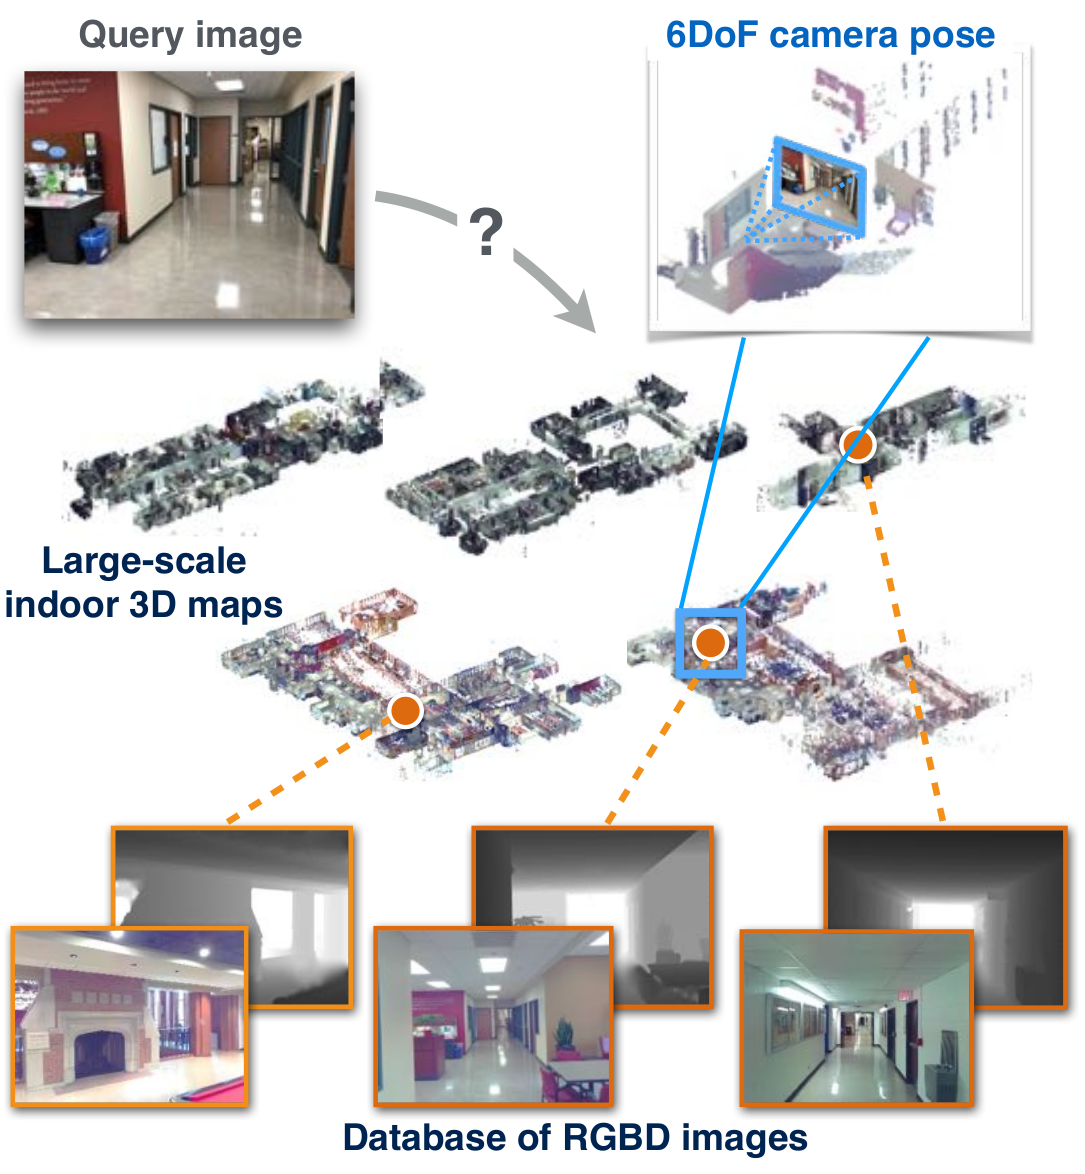
\includegraphics[width=.5\textwidth]{../graphics/inloc.png}
    \caption[InLoc explained]{Given a database of geometrically-registered RGBD images, InLoc predicts
    the 6~DoF camera pose of a query RGB image by retrieving candidate images, estimating candidate camera poses, and selecting
    the best matching camera pose. Image taken from~\citet{InLoc}.}\label{fig:inloc_intro}
\end{figure}

All of illumination changes~(1), textureless areas~(3) leading to lack of sparse local features, such as SIFT~\citep{SIFT},
repetitive elements in indoor settings~(4) leading to similar repetitive features being produced, and even viewpoint changes~(5)
are overcome by utilizing multi-scale dense CNN features computed densely on a regular grid by NetVLAD~\citep{NetVLAD}.
These features are used for database image retrieval, as $N=100$ best matching images are chosen based on sorted
normalized L2 distances of the extracted database feature vectors and the query feature vector.

In the next stage, candidate images are re-ranked by another feature matching in the geometric verification process and
pose estimation. Firstly, features are extracted by VGG~\citep{VGG16} model on conv5 and subsequently on conv3 layer
restricted by previously found matches are used for finding geometrically consistent sets of correspondences with
RANSAC~\citep{RANSAC}. Based on the number of RANSAC inliers, top $M = 10$ candidate database images are kept.
It is to be noted that these features are obtained with no additional computation burden as VGG is used internally
by NetVLAD. As database images used as input to the method are RGBD and hence they have associated 3D points, the
query camera pose is then estimated by finding pixel-to-pixel correspondences between the query and the top
$M$~database images followed by P3P-LO-RANSAC~\citep{P3PLORANSAC}.

To further cope with self-similarity found in indoor locations, counting the number of inliers
as positive evidence to decide whether two views are taken from an exact location is not the
only decisive criterion. Negative evidence is also used in the form of the portion of the view
rendered from the candidate query pose that does not match the query photo. Authors of the paper
refer to this as \emph{explicit pose estimate verification based on view synthesis}. Verification
is done pixel-wise to obtain consistent and inconsistent pixels between the render and the query photo.
To keep invariance to illumination changes and small misalignments, pixel comparison operates with RootSIFT
local patch descriptors~\citep{RootSIFT}. The final image-render similarity is the median of descriptor distance
across the entire image while ignoring areas with missing 3D structure resulting in background-filled regions in renders.

This thesis further examines the view synthesis part of the verification process as it changes the rendered source imputed
to the RootSIFT descriptor computation process. In further chapters, three rendering
techniques alternative to the baseline \verb|GL_POINTS| rendering approach are described in detail.

The decision to use the InLoc method in the thesis was driven by the fact that it is the first method of its kind,
state-of-the-art of its time that puts basis or plays a role of a baseline for
other subsequent state-of-the-art methods~\citep{PoseCorrection}. Further, its source codes are public\footnotei{,}{\url{http://www.ok.sc.e.titech.ac.jp/INLOC}} whereas a subsequent paper~\citep{InLocRevisited}
presenting some improvements does not provide source codes.

\chapter{Point Cloud Rendering} \label{chap:pcd_rendering}

As stated in~\citet{PointRendering}, using point primitives for rendering has been driven
by two main reasons. Over the years,
there was a dramatic increase in the polygonal complexity of models being rendered, leading to
the overhead of managing and processing extensive mesh connectivity information.
Further, modern 3D scanners (LiDAR, stereo camera setup) or photogrammetry methods (SfM) produce
both geometry and appearance of complex, real-world objects in the form of a point cloud. Points in a point cloud
play the role of (discrete) building blocks for 3D scenes, similar to how pixels are the digital ones for images.

Points are the simplest graphic primitive, generalizing pixels towards irregular samples of
geometry and appearance. They differ from triangles typically used in computer graphics
by carrying all attributes needed for processing and rendering with themselves the same way
as pixels do. That results in transformation of rendering pipeline, the terms vertex and fragment coincide in
one entity. Even though the presence of just one such entity may lead to simpler graphical pipelines,
it is not without issues~\citep{ComputeShaderRendering}.

1) Straightforward points projection leaves empty spaces in the image that need to be filled
for close-up views as it may lead to problems with occlusions and visibility or depth perception---with
less dense sampling, a render can end up with just many points scattered across
the background with no notion of what is closer and farther. Thus, point clouds typically
require a denser sampling compared to triangle meshes. 2) Points do not possess any topology or
connectivity information. This fact is an advantage and disadvantage at the same time, compared to
meshed that contain this type of information, but only as a result of 3D reconstruction
algorithms with point clouds being an input that typically still require some prior assumptions on topology
and sampling. It is, for instance, possible to stream and render point clouds progressively, and
change of topology (e.g., by filtering) is more straightforward than for meshes where one needs to recompute
connectivity information~\citep{PointRendering}. On the other hand, effective point processing typically needs
elaborate data structures, including KD-trees~\citep{KDTree} or spatial hashing~\citep{SpatialHashing}.

Over the years, many approaches have been devised for processing point primitives and tackling the
issues presented in the preceding paragraphs. In the thesis, we take advantage of having point clouds-based
datasets. We found out that for large indoor areas, it may be tricky to come up with sufficiently good
mesh that can be further used for the localization verification step rendering, as it can be seen
in~\cref{fig:mesh_artwin_render}. Proceeding with point cloud-based rendering techniques,
we work with three of them together with the mentioned baseline \verb|GL_POINTS| approach;
see their descriptions in the following sections.

\begin{figure}
    \centering
    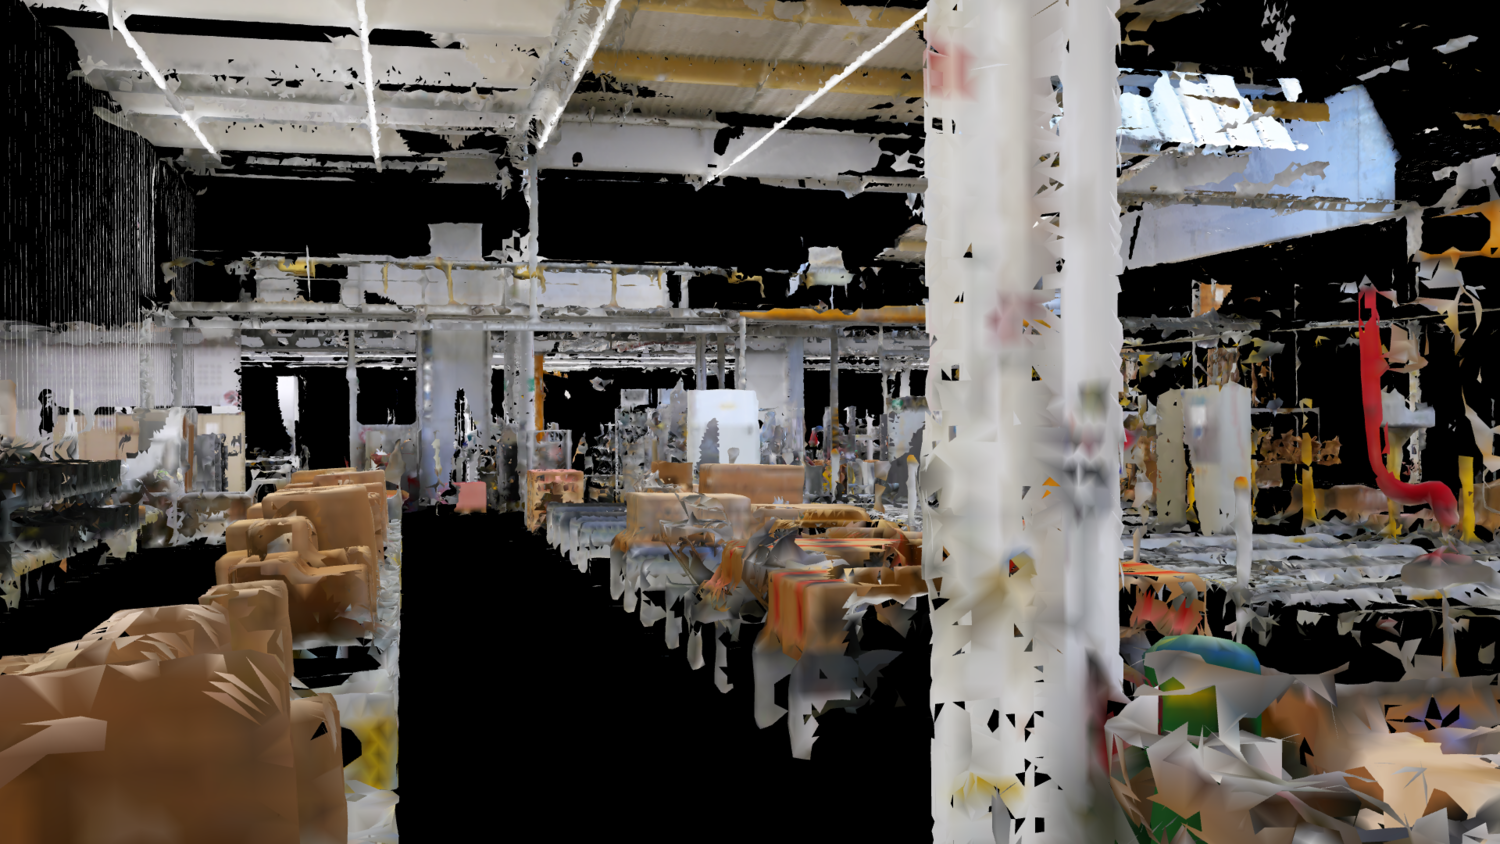
\includegraphics[width=.9\textwidth]{../graphics/0217_mesh_artwin_render.png}
    \caption[ARTwin mesh rendered view]{A render of one of the meshes created from the raw datasets' point cloud, camera pose is the same
    as for~\cref{fig:pyrender_artwin_render}. The mesh was created
    semi-manually, meaning that boxes, for instance, were meshed separately and then placed at the right
    place of the resulting mesh. We can see some disadvantages of using meshes in complex environments.
    Despite long processing time and laborious manual work, the result is not compelling compared to renders
    using point primitives.}\label{fig:mesh_artwin_render}
\end{figure}

\section{Related Work}

\citet{SOTARendering} defined \emph{rendering} as transforming a scene definition, including some of the cameras,
lights, surface geometry, and material, into a simulated camera image. The process can be organized in two
ways~\citep{marschner2021fundamentals}. \emph{Object-order} rendering considers each object; for such,
all the pixels it influences are found and updated. In \emph{image-order} rendering, the loop
goes the other way round, each pixel is considered, and for such, all the objects that influence it are found, and
the pixel value is computed. From these two approaches, image-order rendering is simpler to implement and more capable in the
effects that can be incorporated and usually (though not always) takes more execution time compared to the second approach.
Object-order rendering is also known as \emph{rasterization}, whereas under
\emph{image-order} rendering, there are more possible approaches, such as ray-casting and ray-tracing.\\

Rasterization is typically hardware-accelerated because it has good memory coherence~\citep{SOTARendering}, which is also
one of the reasons for one of the previous claims about execution speed comparison. (Though modern GPU cards already have
hardware support for ray-tracing as well\footnotei{.}{\url{https://developer.nvidia.com/rtx/ray-tracing}}) The rasterization,
as a representative of the object-order methods, requires an explicit scene representation, such as mesh or point cloud, whereas the other
methods work with both implicit and explicit representations.\\

Ray-casting and ray-tracing are, in some sense, orthogonal methods within image-order realm; see~\cref{fig:casting_tracing}.
Ray-casting computes a ray (coming from the camera center
through a specific pixel of the screen) intersections with the representation of the scene to project the scene onto the screen.
In ray-tracing, the primary ray is considered to be coming from the scene, through the screen to the camera center, conveying
color information gathered from all physics-based interactions of light with objects in the scene. Reflections and refractions
are simulated by recursively casting new rays from the intersections with the geometry~\citep{Whitted1979AnII}. The advantage
of this rendering process is the realism of the simulation of real-world optical effects.
While rasterization and ray-casting are a simple, one-way
processes, ray-tracing is an inherently recursive problem. Hence it is a more complex task.

\begin{figure}
    \centering
    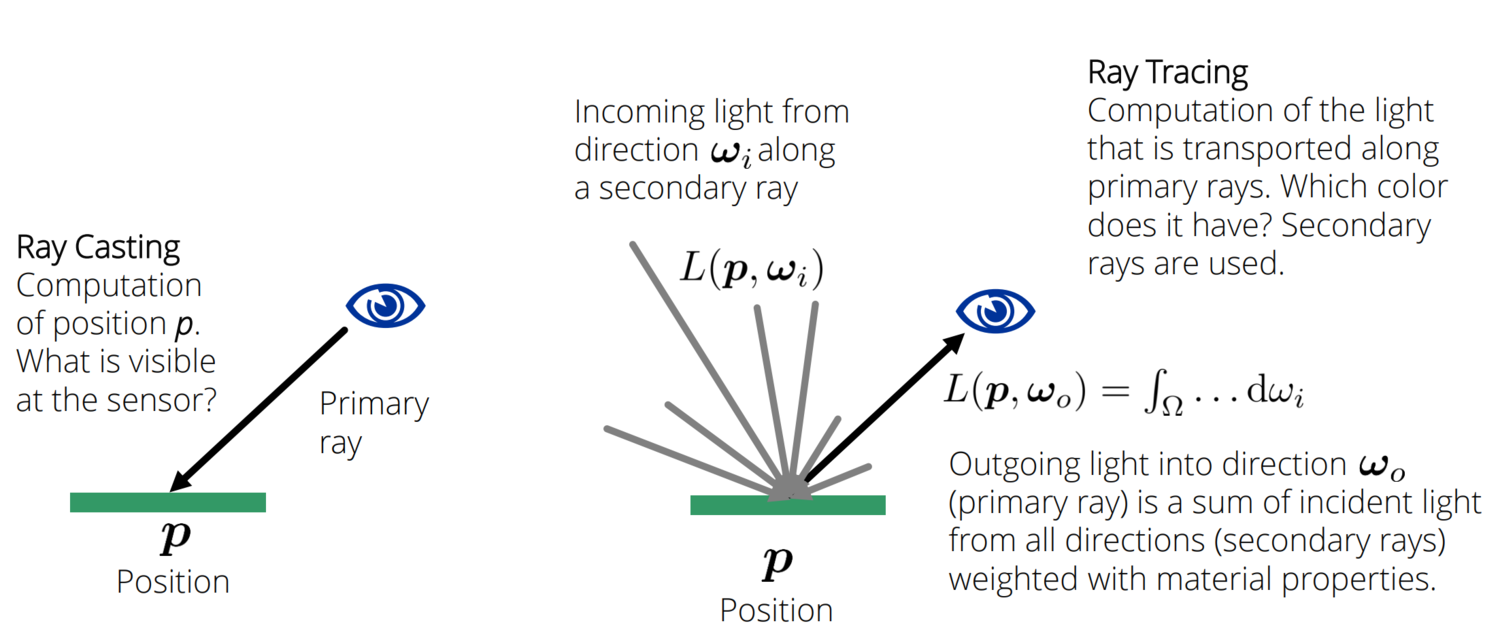
\includegraphics[width=.9\textwidth]{../graphics/casting-tracing.png}
    \caption[Ray-casting vs. ray-tracing]{A demonstration of the difference between
    ray-casting and ray-tracing, together with an illustration of the recursive nature
    of the ray-casting algorithm. Taken from~\url{https://cg.informatik.uni-freiburg.de/course_notes/graphics_01_raycasting.pdf}.}\label{fig:casting_tracing}
\end{figure}

For rendering points with the classical approaches, surface splatting was proposed as a forward-projection approach that uses a z-buffer
algorithm for visibility resolution of points that are exchanged for oriented ellipses. Splatting can process point clouds
without additional acceleration data structures such as spatial hierarchies, which are
often required in ray-tracing approaches~\citep{PointRendering}. The initial article is mainly
a mathematical model and a CPU demonstrator that was later revisited by several papers that enhanced some of its
features and ported it to GPUs~\citep{Splatting2, Splatting3, Splatting4, Splatting5, Splatting6}.
Splatting can also be enriched with ray-tracing again to simulate more complex visual effects~\citep{SplattingTracing}.
Also, further GPU-related enhancements were proposed with better data structures suited for the usage~\citep{SequentialTrees}.\\

Another family of methods takes a vastly different approach than the classical rendering described
above---while traditional computer graphics
methods focus on modeling scenes from a physics perspective, simulating light transport and other effects,
machine learning can be used for modeling the distribution of real-world imagery. The models utilized for this task
are called generative models, successors of the work on \emph{Generative Adversarial Neural Networks}
(GANs)~\citep{GAN}, and can generate high-resolution images~\citep{ICLR, ICLR2} or videos~\citep{VPT, CDS}.
More specifically, the field of so-called neural rendering
combines generative machine learning techniques with knowledge from classical computer
graphics. It is defined as \uv{deep image or video generation approaches that enable
explicit or implicit control of scene properties such as illumination, camera parameters, pose, geometry, appearance,
and semantic structure}~\citep{SOTARendering}. GANs produce \emph{random}, realistically-looking images that resemble
the training set~\citep{DGM} statistically. As the definition of neural rendering states, user controllability
is important---if used by an artist, outputs reflecting design ideas are preferred over some random imagery.
For applications in the neural rendering field, GANs thus needed to be extended by the conditioning of output
to enable guidance of the rendering process.

Further citing~\citet{SOTARendering}, neural rendering techniques can be classified along different axes:
\begin{itemize}
    \item \textbf{Control}. This axis distinguishes neural rendering approaches based on
    what properties from the definition are controllable and how they condition
    the network's output. A general solution enabling to control everything is an open
    research problem. Typically only a subset of controllable properties is approached
    in subproblems like novel view synthesis, relighting, or face and bodies animation.
    The conditioning can be performed by passing the scene parameters as input to some network
    layer or concatenating them to activations of an inner one, by tiling scene parameters over
    all pixels of an input image resulting in packed input volume, it can also employ
    an image-to-image transformation DNN that fuses \uv{guide image} into to the output one.
    Also, a more traditional approach uses scene parameters as an input to a graphical layer.
    \item \textbf{Computer Graphics Modules}. The separation along this axis is based on how much
    of the classical rendering pipeline is integrated into the specific method. The simplest way
    to achieve that is to use a non-differentiable computer graphics (CG) component in the network
    architecture, which would present the render as an input to subsequent differentiable layers of a given architecture.
    When the module is at the beginning of the architecture, the task transforms into
    well-researched image-to-image translation. Fully differentiable CG modules also exist.
    \item \textbf{Explicit vs. Implicit Control}. Here, the criterion is based on a type of
    control signal. Explicit control from a user perspective means manual editing capability
    of scene parameters in a semantically meaningful manner. By implicit control, a representative
    sample as input is meant. The difference also translates to training data as explicit control
    needs richer annotations, whereas implicit one performs well with less supervision.
    \item \textbf{Multi-modal Synthesis}. Not only from an art perspective, often it is beneficial to have
    multiple outputs from which a user can choose. Especially when only a subset of scene properties is
    controllable, within the rest, there lies an output space of possible results from which a given model
    can sample. This sampling capability adds complexity to the architecture, requiring some
    stochasticity or structured variance built-in, leading to GAN or variational auto-encoders (VAEs) variants.  % TODO clanek
    \item \textbf{Generality}. Does the rendering approach perform well over multiple
    scenes or objects without retraining the underlying model? Object-specific approaches
    still produce higher quality outputs at the cost of lengthy per-instance retraining. General models
    are still an open research area.
\end{itemize}

Methods spread across this classification landscape solve various subtasks of the neural rendering field.
Given the model this thesis utilizes, the novel view synthesis task is described next.\\

\emph{Novel view synthesis} generates a view of a
scene, represented by a fixed set of input images, from previously unexplored camera poses. Challenges tied to this task are inferring the scene's 3D
representation, given sparse observations in the form of images and deducing of occluded
or unseen areas of the scene. For the scene reconstruction, the aforementioned SfM is being utilized, followed by
MultiView Stereo (MVS)~\cite{MVS1, MVS2} or variational optimization~\cite{VarOpt}.

The classical computer vision approach towards novel view synthesis utilizes so-called image-based rendering (IBR)
methods~\citep{IBR1, IBR2, IBR3, IBR4} where views from new viewports are generated by warping input pixels into the
outputs using proxy geometry. These methods are sensitive to the scene database size as IBR may fail with insufficient number of source photos, resulting in ghosting-like artifacts and holes~\citep{SOTARendering}. These approaches
also do not handle multiple appearances well~\citep{NRIW}. Neural networks and
rendering alternative approaches have been proposed to mitigate these issues, such as~\citet{NR1, NR2, NRIW, InvSfM, FVS, SVS}.
These methods build on IBR and image-to-image translation using explicit scene models. Learned implicit
scene representation can be leveraged as well, see the Neural Radiance Fields~\citet{NERF, NERF2}
and~\citet{SceneRepr}.

The Neural Radiance Fields, together with the Gaussian Splatting neural model~\citep{kerbl3Dgaussians}
combining the neural field with the splatting idea explored in the thesis represent the recent progress
in the field nicely, alleviating some of the issues of the previous models. However, they were not yet
available when the work on the thesis was started, they are not considered.


\section{Neural Rerendering In the Wild}

According to the neural rendering techniques classification, the \emph{Neural Rerendering In the Wild} (NRIW) method~\citep{NRIW}
can be shortly described as a method explicitly controlling camera parameters, pose, and illumination, using
non-differentiable CG module preprocessing an input, producing multiple modalities, and being scene-specific.
More specifically, the authors tackle what they define as \emph{total scene capture} with a deep generative model that can
\begin{enumerate}
    \item perform novel view synthesis for a given scene,
    \item can capture and render various appearances of the scene, e.g., all
    weather and illumination conditions,
    \item and finally, it should understand the location and appearance of transient objects
    in the scene, such as people and vehicles, for reproducing or omitting them.
\end{enumerate}

Following~\citep{Bastien} in need of realistic point cloud renders, we utilize the model for
both indoor and outdoor rendering.

\uv{In the Wild} is related to unstructured photo collections from the internet NRIW can work with.
The method starts with building a proxy explicit 3D colored point cloud representation from a collection of
scene photos~$\{I_i\}$ by utilizing Structure-from-Motion (SfM) and MultiView Stereo (MVS) implemented by
COLMAP~\citep{schoenberger2016sfm, schoenberger2016mvs}. Authors prefer point clouds over generating a mesh
in a possible next step, even though meshes generate more complete renderings, as meshes \uv{also tend to contain pieces of misregistered floating geometry which can occlude large regions of the scene}.

In the next stage, an aligned dataset of deferred-shading deep buffers $B_i$ is generated. Such a buffer,
in general, may contain per-pixel albedo, normal, depth, and any other derivative information. Authors use
a combination of rendered and real images~$\{I_i\}$, together with albedo and depth representations, all
depicting the same view. By the rendered image, a point splatting with a z-buffer with a radius of 1 pixel
render of the scene point cloud from a position $v_i$ recovered for the respective real image $I_i$ by SfM
is meant. Even though this may resemble an image-to-image translation paradigm, it is not the case as
such a model is uni-modal, not including appearance modeling. Image-to-image translation also fails to
understand transient objects in the scene.

The aligned dataset is used to train a multimodal image translation model. Its goal is to learn
a latent appearance vector~$z^a_i$ that captures variations in the output domain~$I_i$ that cannot be
inferred from the input domain~$B_i$. The method computes~$z^a_i$ as~$E^a(I_i, B_i)$, where~$E^a$ is
an appearance encoder of input~$I_i$ and~$B_i$ (the buffer is used for allowing the network to learn
more complex appearance models by correlating the lighting in the real image with scene geometry in the
corresponding buffer). Lastly, a rerendering network~$R$ produces a scene rendering conditioned
on both deep buffer~$B_i$ and the latent appearance vector~$z^a_i$. \cref{fig:nriw} presents a visual
overview of the process.

\begin{figure}
    \centering
    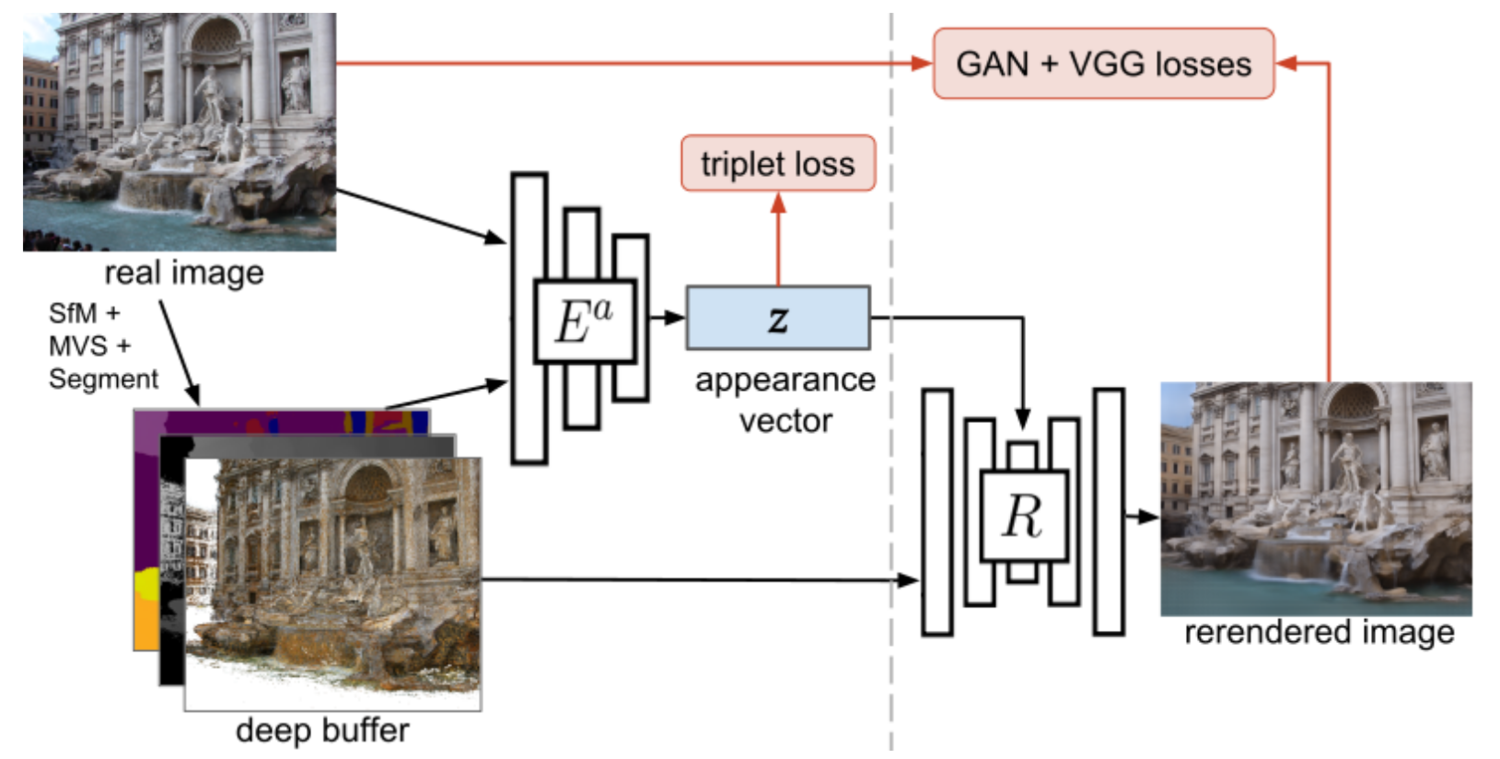
\includegraphics[width=.9\textwidth]{../graphics/nriw.png}
    \caption[NRIW model training]{Both neural networks are trained in a staged approach
    that pre-trains the appearance encoder~$E^a$ using a triplet loss, subsequently the
    rerenderer~$R$ is trained with standard reconstruction and GAN losses (right), and
    finally, fine-tuned together with~$E^a$. Taken from~\citet{NRIW}.}\label{fig:nriw}
\end{figure}

The training process works as follows---to stabilize the joint training of~$R$ and~$E^a$, and improve
the model expressiveness, pre-training the appearance encoder~$E^a$ on a proxy task is first performed.
In a staging manner, rendering network~$R$ is then trained using fixed~$E^a$ weights, allowing~$R$ to
find the correlations between output images and the embedding produced by the proxy task~$E^a$ training.
Finally, both networks are jointly fine-tuned.

The appearance pre-training works on a proxy task that optimizes
embeddings of the input images in the appearance latent space based on a suitable distance metric. Similar images under the metric should also have similar embeddings. The metric itself should ignore viewport as appearance is independent of it.
For that, authors use neural style-transfer triplet loss---for each image~$I_i$, sets of~$k$ closest and
farthest neighboring images with respect to the metric below are found. From those, one positive~$I_p$
and one negative~$I_n$ image is sampled, respectively. The loss then is:

$$\mathcal{L}(I_i, I_p, I_n) = \sum_j \mathrm{max}\left(\lVert g_i^j-g_p^j\rVert^2 - \lVert g_i^j-g_n^j\rVert^2 + \alpha, 0\right)\,,$$

where~$g_i^j$ is the Gram matrix of activations at the~$j$-th layer of a VGG network of image~$I_i$,
and~$\alpha$ is a separation margin.

Lastly, semantic conditioning performed by concatenating a semantic labeling~$S_i$ of
image~$I_i$ to the deep buffer~$B_i$ is used to account for transient objects. The authors argue that
it discourages the appearance encoder network from encoding variations caused by the location of
transient objects in the appearance latent space or associating such objects with specific viewports.

\section{Surface Splatting}

Surface splatting, presented by~\citet{SurfaceSplatting}, is an efficient technique for rendering high-quality
images of point clouds (point-sampled surfaces), supported by rigorous mathematical analysis around
resampling. In contrast to ray-tracing, it is a forward-projection approach that uses z-buffer to
resolve visibility. It can avoid aliasing artifacts brought alongside discretizing otherwise
continuous space by a screen space formulation of the Elliptical Weighted Average (EWA) filter for
irregularly spaced point samples without global texture parameterization.

It can be seen as a resampling process in signal processing~\citep{PointRendering}, effectively the method
strives to reconstruct initially hole-free surfaces sampled in the form of a point cloud. To do so, the method
uses a combination of an object-space reconstruction filter and a screen-space filter for each point primitive.
The mathematical object-space reconstruction filter (\emph{footprint function}~$\rho_i(\mathbf{x})$ of a point~$\mathbf{x}$)
resembles typically an elliptical disk, a so-called splat whose position, orientation, and axes are usually
chosen to provide a good approximation to the underlying source geometry. After a perspective projection of all splats
to the screen space, the EWA filter mentioned above is used to avoid frequencies higher than the Nyquist frequency
of the pixel sampling grid, and all contributions from the overlapping splats are combined.

\SaveVerb{term}|GL_POINTS|
\begin{figure}
    \centering
    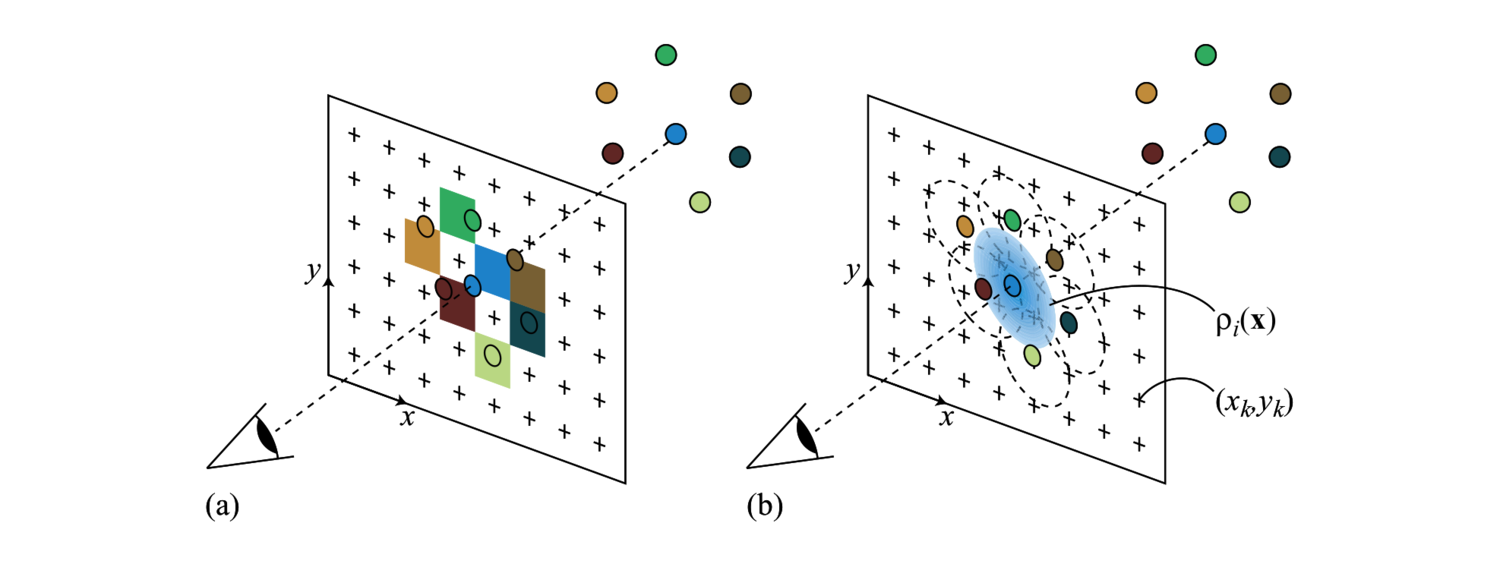
\includegraphics[width=.9\textwidth]{../graphics/splatting_principle.png}
    \caption[Surface splatting compared to simple projection]{Point rendering
    by surface splatting compared to a naive approach that is used, for instance,
    by \protect\UseVerb{term} OpenGL primitive. (a) Naive forward projection and rendering of point samples
    assigning the projected point's color to the closest pixel in the screen space. (b) By splatting footprint
    functions, each pixel gets color decided upon a combination of contributions scree-space neighboring points.
    Taken from~\citet{PointRendering}.}\label{fig:splatting_principle}
\end{figure}

The basic idea of splatting compared to a naive approach is shown in~\cref{fig:splatting_principle}.
The naive method does not work generally as it leads to holes in reconstructed surfaces in the rendered image
if the surface is not sampled with sufficient frequency. Also, another disadvantage happens when more than
one point gets projected to the same closest pixel---then the rendering result depends on the order in
which the points are processed. Surface splatting alleviates the problems by distributing the color of
each projected point among more neighboring screen-space pixels with a suitable footprint function.
The desirable footprint function is usually smooth, decays quickly with increasing
distance from the projected center, and has local support as indicated by the ellipses in~\cref{fig:splatting_principle}.

For a single channel of a possible multiple-channel (taken independently) image, image function~$\phi(x, y)$
taking a pixel position and returning color could be defined according to previous thoughts as

\begin{equation}\label{eq:simple_splatting}
\phi(x, y) = \sum_i c_i\rho_i(x, y)\,,
\end{equation}
where the sum is carried over the indices of all points~$\{\mathbf{p}_i\}$ of the surface, $\rho_i$ are individual
footprint functions, and~$c_i$ are channel color values of a given point.

The definition~\cref{eq:simple_splatting} has an issue with reproducing surfaces with constant color and thus can
lead to visible artifacts. Also, footprint functions are truncated to finite support. Both leads to the below presented
normalized image function used by surface splatting

\begin{equation}\label{eq:normalized_splatting}
\phi(x, y) = \sum_i c_i\frac{\rho_i(x, y)}{\sum_k \rho_k(x, y)}\,.
\end{equation}
The image function defined by~\cref{eq:normalized_splatting} leads to a two-pass algorithm for
rendering~\cref{algo:splatting}. In the first pass, all points are iterated over and their splat
footprints~$\rho_i$ and channel values~$c_i$ are computed. The footprint functions are evaluated at each pixel, or
rasterized, and their contributions are accumulated in a buffer. At each pixel~$(x, y)$,
the buffer stores the sum of the weighted contributions from the right side of~\cref{eq:simple_splatting},
normalization factor sum from the denominator of~\cref{eq:normalized_splatting} and the depth for z-buffering.
In the second pass, all pixels are processed by normalization of the accumulated contributions by the accumulated
normalization factor.

\begin{algorithm}[t]
	\caption{Pseudocode of the splatting algorithm.}\label{algo:splatting}
	\begin{algorithmic}[1]
		\Procedure{splat\_rendering}{p[], c[], w[], z[]}
			\For{all points i \textbf{in} p[]}
					\State rho\_i $\gets$ footprint(p\_i)
					\State c\_i $\gets$ shade(p\_i)
                        \State rasterize(rho\_i, c\_i, c[], w[], z[])
			\EndFor
			\For{all points [x, y]}
                        \State c[x, y] /= w[x, y]
			\EndFor
		\EndProcedure
	\end{algorithmic}
\end{algorithm}

How usable footprint functions are found and look is beyond the scope of this work as it requires
signal-processing theory, Gaussian functions, and the Nyquist theorem. We utilize
a GPU implementation by Sebastian Lipponer\footnotei{.}{\url{https://github.com/sebastianlipponer/surface_splatting}}

\section{Ray Marching with Signed Distance Fields}

This method is an example of a ray-casting approach, in which a finite series of steps along
a ray cast from a camera through a pixel is undertaken, until the ray hits an object or
the maximum number of permitted steps is exceeded. This very simple idea is fundamental in
computer graphics and dates back to works like~\citet{RayMarching, Hypertexture}. Building
on the idea, many effects, such as lights, shadows, and transparency, can be incorporated, to
name a few~\citep{RealTimeRendering}. This thesis implements a variant of the method using
\emph{signed distance functions} (SDF).

In a given scene consisting of solid bodies, a \emph{signed distance function} is a scalar
function~$S(P)$ defined at every point~$P$ in a (2D or 3D) space, such that

\begin{equation}\label{eq:sdf_def}
\begin{array}{ll}
S(P) = 0 & \text{when it is on the surface of a body,}\\
S(P) > 0 & \text{when it is inside any body,}\\
S(P) < 0 & \text{when it is outside all bodies~\citep{SDF}.}
\end{array}
\end{equation}

A \emph{scene SDF} defines the scene implicitly. An \emph{object SDF} is the SDF of a scene containing
only that one object. Object SDFs can be computed analytically for simple shapes; see
work of Inigo Quilez\footnotei{,}{\url{https://iquilezles.org/articles/distfunctions}}
or tabulated in grids, octrees, or other spatial data structures. A scene SDF can then be constructed
by combining SDFs of objects in the scene. For simple analytically-describable shapes, an
insight into how such a scene can be built may be given through Constructive
Solid Geometry (CSG), a method of creating complex geometric shapes from simple ones via boolean
operations, see the left of~\cref{fig:rm}. This process has its mirror in combining SDFs; see code example in~\cref{code:sdfs}.
As an example, an SDF for the simplest 3D object, a sphere positioned at the origin and with a defined radius,
is \verb|SDF_sphere(vec3 pos) -> length(pos) - RADIUS|. In general, SDF does not need to be based on Euclidean distance
and may be exact or approximate. The only theoretical requirement is~\cref{eq:sdf_def} and from a practicality perspective,
evaluation of such a function should be reasonably quick.
The algorithm utilizing a scene SDF is outlined in~\cref{algo:marching}. The visual representation of
the simplest form of the algorithm proceeding along a ray is to be found in the right of~\cref{fig:rm}.

\begin{lstlisting}[language=Python,caption=Code example showing how SDFs of simpler object can be combined together to gradually build a scene SDF., label=code:sdfs]
def SDFintersect(obj1_SDF, obj2_SDF):
    return max(obj1_SDF, obj2_SDF)

def SDFunion(obj1_SDF, obj2_SDF):
    return min(obj1_SDF, obj2_SDF)

def SDFdifference(obj1_SDF, obj2_SDF):
    return max(obj1_SDF, -obj2_SDF)
\end{lstlisting}

\begin{figure}
	\centering
	\begin{subfigure}{.5\textwidth}
		\centering
		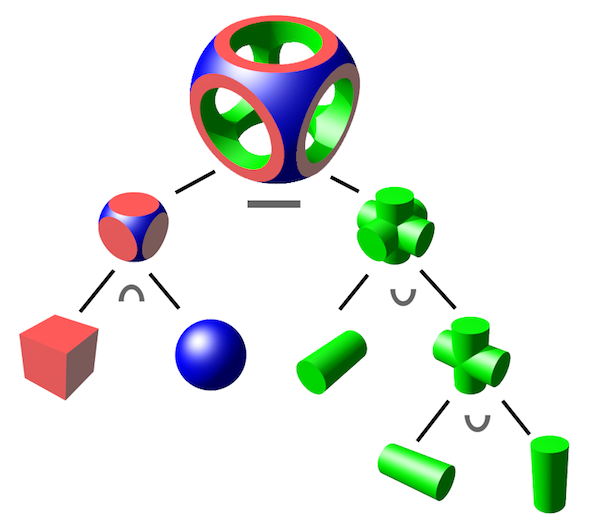
\includegraphics[width=.9\textwidth]{../graphics/csg.png}\label{fig:csg}
	\end{subfigure}%
	\begin{subfigure}{.5\textwidth}
		\centering
		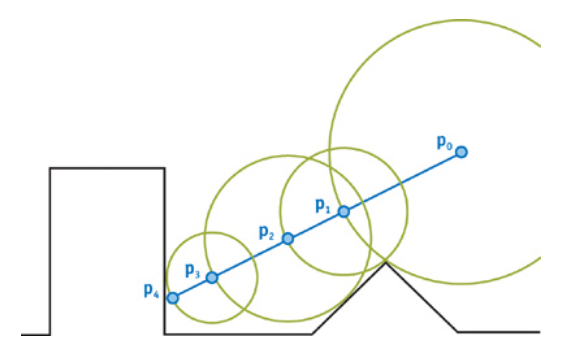
\includegraphics[width=.9\textwidth]{../graphics/marching.png} \label{fig:marching}
	\end{subfigure}
	\caption[Ray Marching and Constructive Solid Geometry]{Left: CSG is
        built upon three primitive operations: intersection ($\cap$),
        union ($\cup$), and difference ($-$).
        Taken from~\url{https://en.wikipedia.org/wiki/Constructive_solid_geometry}. Right: Demonstration
        of ray marching where at each step algorithm proceeds along given ray by a distance to the
        closest surface as it is a safe way how to find a hit, based on some threshold distance.
        Taken from~\url{https://jamie-wong.com/2016/07/15/ray-marching-signed-distance-functions/}.} \label{fig:rm}
\end{figure}

In this thesis, we utilize scene representation relying on translated sphere SDFs with radii precomputed beforehand
to be dependent on the distance to the closest neighbor for a given point primitive. Scene SDF for such a
scene would be then a minimum of all point SDFs in the scene (following again~\cref{code:sdfs}). This naive
declaration is not scalable to millions of points a scene produced by a LiDAR or SfM may contain, even though
only the simplest point primitives are used for the rendering process. To increase significantly rendering performance
with sufficient reality reproduction capabilities, we take advantage of a spatial 3D KD-tree~\citep{KDTree}
implemented in NVIDIA CUDA\footnote{\url{https://developer.nvidia.com/cuda-toolkit}} toolkit that can quickly
return the closest point for a given location. Since the exact sphere SDF contains its radius and KD-tree built
on top of the source point cloud returns the distance to the sphere center (point) itself, not the distance to the sphere's surface,
we take~$N$ closest points, instead of just one, compute exact SDF for those with their respective radii, and then take the point
at the minimal distance determined. The same KD-tree is pre-build once at the start of the rendering process and
is also used for radii computation instead of computing those exhaustively.


\begin{algorithm}[t]
    \caption{Pseudocode of the ray marching with SDF.}\label{algo:marching}
    \begin{algorithmic}[1]
        \Procedure{ray\_march}{ray\_origin, ray\_direction}
            \State dist $\gets$ 0
            \For{i \textbf{in} range(MAX\_STEPS)}\Comment{Hyperparameter to stop traversal}
                \State current\_pos $\gets$ ray\_origin $+$ dist $*$ ray\_direction
                \State closest $\gets$ SDFscene(current\_pos)
                \If{closest.dist $<$ MIN\_HIT\_DIST}\Comment{Float comparison}
                    \State \textbf{return} closest.color
                \EndIf
                \If{dist $>$ MAX\_DIST}\Comment{No hit along the ray}
                    \State \textbf{return} BACKGROUND\_COLOR
                \EndIf
                \State dist $\gets$ dist $+$ closest.dist
            \EndFor
        \EndProcedure
    \end{algorithmic}
\end{algorithm}

\chapter{Camera Pose Verification}

In the chapter, datasets, their transformations, and experiments performed upon them with
the introduced methods' implementations are all presented. We use the generalized InLoc
pipeline with a modified pose verification step. The synthesized image leveraged for
pixel-wise computation of similarity with the given query image is swapped with views
generated by renderers presented in the preceding chapter, depicting the scene's point
cloud from estimated query positions. Apart from how the synthesized image is generated,
the rest of the verification process is then performed according to the original article,
using namely RootSIFT descriptors.\\

While discussing concrete details of datasets' definitions and algorithms' inputs, more
technical aspects are taken into account---among them, of utmost importance are
conventions used by coordinate systems in which points of explicit scene representations
are expressed/expected to be and by matrices related to cameras taking database images.
These pose a crucial difference between what a dataset provides, or localization pipeline
expects and must be addressed by implementation to obtain valid localization results.

\begin{figure}
    \centering
    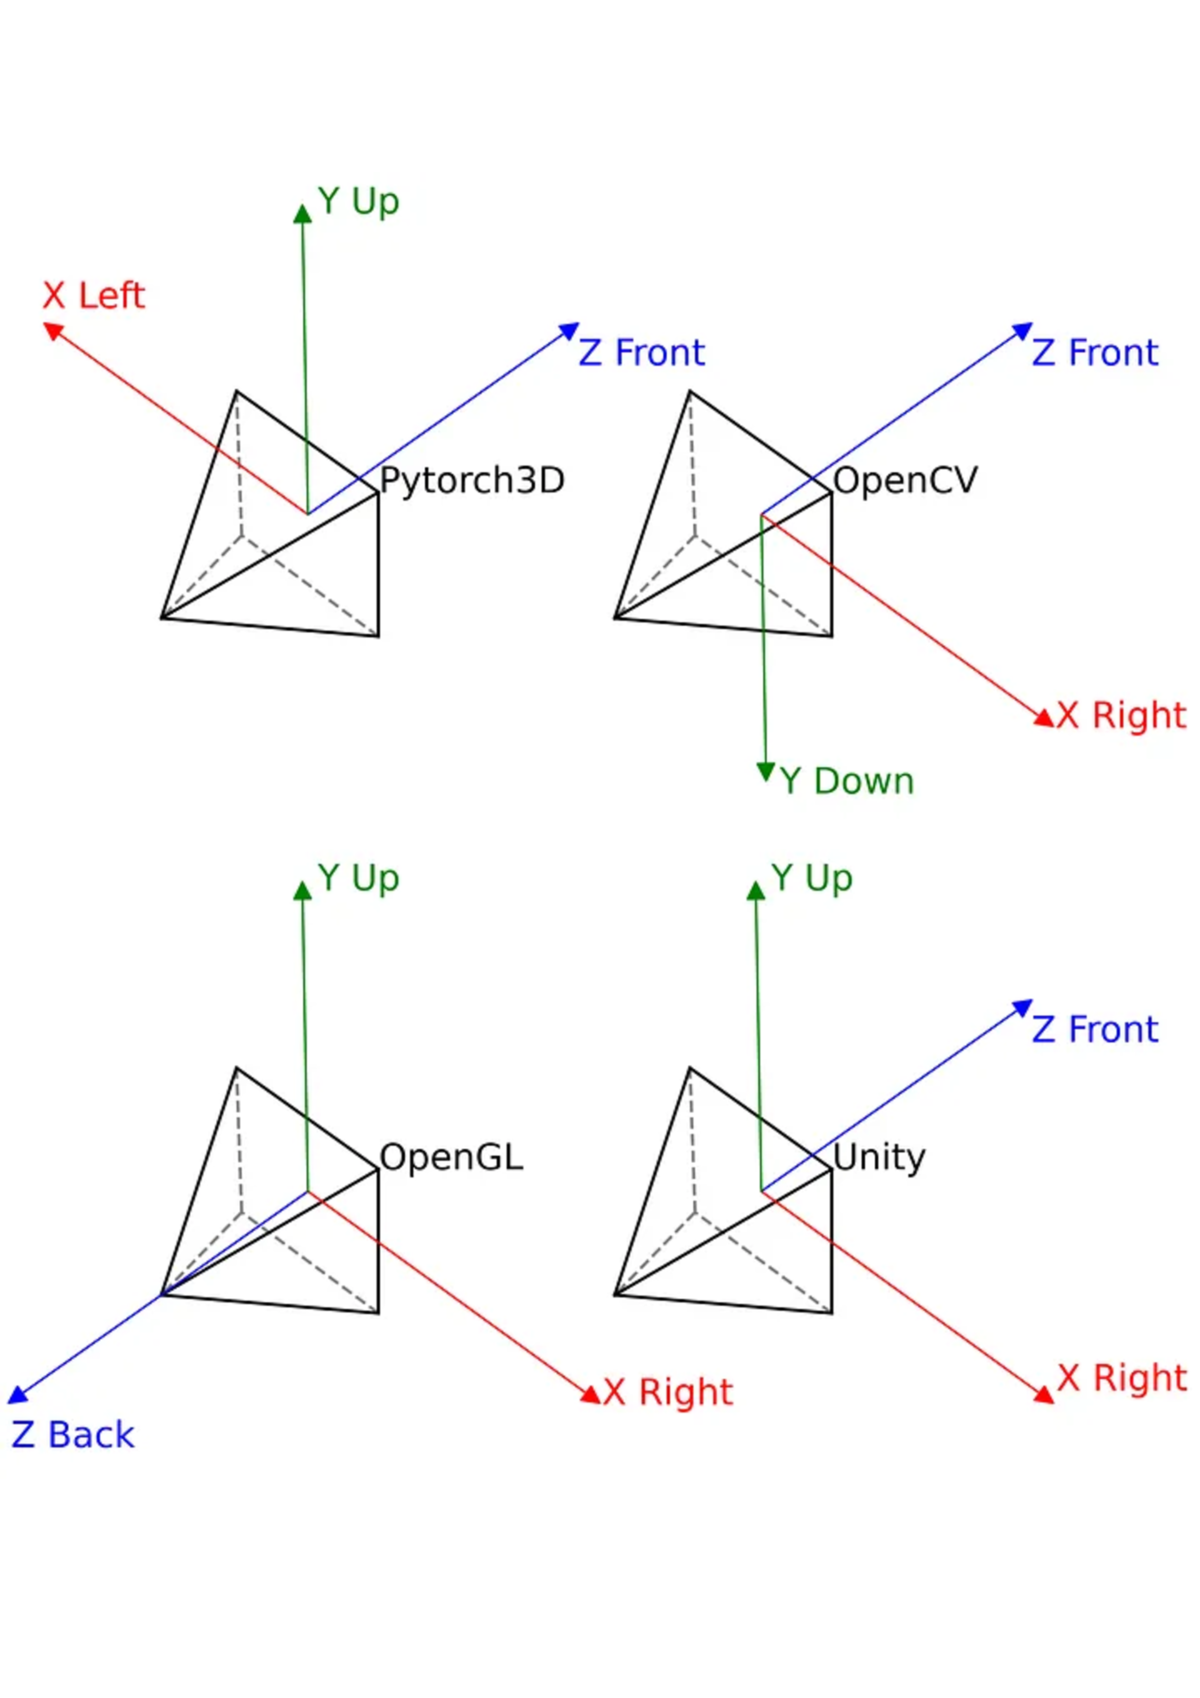
\includegraphics[width=.7\textwidth]{../graphics/cs_conventions.png}
    \caption[Examples of various camera\,/\,coordinate frame conventions]{
    Examples of various camera\,/\,coordinate frame conventions used by
    common programmatic tools in fields dealing with computer graphics.
    Taken from~\url{https://medium.com/check-visit-computer-vision/converting-camera-poses-from-opencv-to-opengl-can-be-easy-27ff6c413bdb}.}\label{fig:cs_conventions}
\end{figure}

Coordinate system conventions address the decision of assigning positive directions,
labels, and meanings in the human sense (up, right, forward) to the orthogonal frame of a
3D space, because without that an oriented triplet representing a point is meaningless.
These conventions can be arbitrary depending on whether they come from computer vision,
rendering, or another field. Examples of such conventions, linked to standard computer
graphics libraries/tools that use/expect them, can be found in~\cref{fig:cs_conventions}.
In this thesis, computer vision and rendering conventions are used. In the
figure~\cref{fig:cs_conventions}, these are found alongside OpenCV and OpenGL labels,
respectively. Even though both are right-handed, they understand x, y, and z point
components differently.  In rendering, the positive x-axis points to the right, the
positive y-axis up, and the positive z-axis towards a viewer looking at the coordinate
system frame. In computer vision, the positive x-axis points to the right, the positive
y-axis to the bottom, and the z-axis away from the same viewer as before. Transformation
matrices operating over both notations are thus related by inverting the y and z axes
columns. As an example, since a camera in rendering is typically placed along z-xis,
failing to take this relation into account when displaying a 3D model defined in computer
vision notation in a visualization tool that uses rendering notation results in rendering
half-space \uv{away} from the model. For instance, in the case of other notations used by
a produced model, a rendered view can be somewhat unexpectedly rotated.

Matrix conventions in the context of the thesis are related to terms coming from the
graphics pipeline---\emph{world space} and \emph{view space}. In the case of datasets
described below, world space is a space of the whole scene representation with the origin
and orientation of the coordinate frame chosen arbitrarily in relation to the scene.  The
randomness in the coordinate frame placement is especially true in the case of
SfM-generated scene models, where the algorithm decides these parameters.  When preparing
a model manually, e.g., in the game industry, the frame is typically artificially placed
meaningfully concerning the model produced, e.g., along the outer edges of a cube model.
View space is a space of a camera looking at a portion of the scene---origin is the center
of the camera with the coordinate frame oriented in a specific way alongside the optical
axis of the camera depending on the exact graphics pipeline/tool used.
Visualisation~\cref{fig:cs_conventions} can be used here as well---the square pyramids
depict view frustums of virtual cameras, with the z-axes being their optical axes.

Provided both spaces are same-handed, the matrix inverse relates transformations between
them. In homogeneous coordinates, both transformations are represented by $4\times4$
matrices, and the implementation must correctly distinguish between the actual meaning of
these 16~real numbers, including how the matrix is stored on the disk. We refer to them as
the \emph{view matrix} transforming from world to view space and \emph{camera pose}
representing the opposite, inverse transformation.

\chapter*{Conclusion}
\addcontentsline{toc}{chapter}{Conclusion}

This thesis examines the usage of various rendering techniques in the InLoc
algorithm solving the visual localization problem and its verification step.
The point cloud rendering approaches, and later localization performance are
evaluated on three different dataset types covering both exteriors and
interiors; the InLoc implementation is generalized so that a general dataset,
not only the one that InLoc was released with, can be inputted for localization.

Four different rendering approaches are utilized---as a baseline approach,
the default OpenGL point rendering primitive \verb|GL_POINTS| is used, further,
point splatting and ray marching with signed distance fields are explored.
Finally, aside from the three classical rendering approaches, a neural
rendering deep neural network model is compared with the previous ones. As not
all mentioned renderers were in existence prior to the thesis with sufficient
performance to be able to render point clouds of sizes present in the datasets,
third-party point splatting C++ implementation within a graphical interface is
enhanced with headless rendering capabilities, the capability to read external point
clouds and camera parameters, and output depth information for renders. The ray
marching renderer is implemented in C++ and CUDA from the ground, eventually
reusing the same components from the splatter enhancements. To the best of our knowledge,
previously, there were no such implementations with these capabilities being able
to render tens of millions of points in a reasonable time.\\

We considered the renderers from various angles---rendering performance from visual
and statistical perspective, from computational performance, and finally, from
influence on the localization performance. We show that aside from computational
perspective, the four renderers split roughly into three groups: the predominantly
least performant algorithm is Pyrender, followed by the Splatter and Marcher
implementations with the NRIW model on the top.

\emph{Pyrender} suffers from its slower
implementation in Python and from the primitive it uses as the points have fixed
size in the screen space, which defies perspective drawing principles, leading to
visual artifacts in the form of occlusion problems.

\emph{Splatter} and \emph{Marcher} are less easy to separate. Their principle
is similar as it uses diameters assigned to points and renders them as splats or
spheres. In practical use cases, there are differences, however.
The Splatter requires a normal vector per point on top of diameters to
properly put a face to the splats. In the case of all datasets explored in the
thesis, we did not encounter a situation where a dataset would simultaneously
explore one space from the inside and outside. However, if this happens, Splatter
would require additional functionality to dynamically compute normals per view
or switch directions based on some condition fulfillment. On the other hand,
Splatter shows less dependency on the view frustum contents, whereas Marcher
performs much less consistently. For some views, the rendering time may be
considerably longer than for others. There is room for improvements in the
implementation that may mitigate this issue, including the possible memory caching
boundary hit, causing extremely prolonged rendering times in some cases. Visually,
Splatter can represent corners and edges with less blur. Finally, both
renderers increase the performance of the InLoc pipeline when used for the
dataset's transformation into the InLoc format and for training a neural model
used in the verification step.

The \emph{NRIW} model further pushes localization performance due to its more
realistically-looking rendering capabilities that get exploited in the verification
step of the localization pipeline. The disadvantages and the price for the localization
precision gains are speed, as the model needs, on top of its own slower runtime,
a proxy render of a point cloud from a candidate position generated by another
non-neural renderer, and also its scene dependency that requires training for
every dataset explored. There has been considerable progress in the neural rendering
field since work on the thesis started, so future work may explore these advancements.\\

To summarize, when maximal localization performance is sought, Splatter and Marcher
help the localization pipeline's frontend, together with neural rendering based on the
same. For concrete use cases, other differentiating factors can help to choose a specific
renderer. When the time of answering a localization query is to be minimized, it may be
worth sacrificing some precision by either using the non-neural renderers for the whole
pipeline or, as we show, by lowering the number of points in the scene model that is from
both statistical and visual point of view comparable with the advantage of faster
rendering times. Future work may analyze the effect of lowering the resolution of the
database and query images to inspect the computational performance further.



%%% Bibliography
%%% Bibliography (literature used as a source)
%%%
%%% We employ bibTeX to construct the bibliography. It processes
%%% citations in the text (e.g., the \cite{...} macro) and looks up
%%% relevant entries in the bibliography.bib file.
%%%
%%% The \bibliographystyle command selects, which style will be used
%%% for references from the text. The argument in curly brackets is
%%% the name of the corresponding style file (*.bst). Both styles
%%% mentioned in this template are included in LaTeX distributions.

% \bibliographystyle{apalike}
% \bibliographystyle{dinat}
\bibliographystyle{plainnat}    %% Author (year)
% \bibliographystyle{unsrt}     %% [number]

\renewcommand{\bibname}{Bibliography}

%%% Generate the bibliography. Beware that if you cited no works,
%%% the empty list will be omitted completely.

\bibliography{bibliography}

%%% If case you prefer to write the bibliography manually (without bibTeX),
%%% you can use the following. Please follow the ISO 690 standard and
%%% citation conventions of your field of research.

% \begin{thebibliography}{99}
%
% \bibitem{lamport94}
%   {\sc Lamport,} Leslie.
%   \emph{\LaTeX: A Document Preparation System}.
%   2nd edition.
%   Massachusetts: Addison Wesley, 1994.
%   ISBN 0-201-52983-1.
%
% \end{thebibliography}


%%% Figures used in the thesis (consider if this is needed)
\listoffigures

%%% Tables used in the thesis (consider if this is needed)
%%% In mathematical theses, it could be better to move the list of tables to the beginning of the thesis.
\listoftables

%%% Abbreviations used in the thesis, if any, including their explanation
%%% In mathematical theses, it could be better to move the list of abbreviations to the beginning of the thesis.
\chapwithtoc{List of Abbreviations}
SfM
DNN
CNN
NN
CG
GAN
VAE
VGG
SDF
CSG

%%% Attachments to the master thesis, if any. Each attachment must be
%%% referred to at least once from the text of the thesis. Attachments
%%% are numbered.
%%%
%%% The printed version should preferably contain attachments, which can be
%%% read (additional tables and charts, supplementary text, examples of
%%% program output, etc.). The electronic version is more suited for attachments
%%% which will likely be used in an electronic form rather than read (program
%%% source code, data files, interactive charts, etc.). Electronic attachments
%%% should be uploaded to SIS and optionally also included in the thesis on a~CD/DVD.
%%% Allowed file formats are specified in provision of the rector no. 72/2017.
%\appendix
%\chapter{Attachments}

%\section{First Attachment}

\openright
\end{document}
